\section{性能試験}
開発したHDR1軸力覚センサの性能を評価するために荷重印加試験を行った.
Fig.~\ref{fig:sensor}に示す荷重印加位置に任意の荷重を印加し, 
その時の金属箔ひずみゲージと半導体ひずみゲージの出力を調べた. 
印加荷重は$0~2.5N$の範囲で$0.5N$刻みに印加した.

実際に製作した力覚センサと実験の様子をFig.~\ref{fig:jissai}示す.
\begin{figure}[h]
  \centering
  \begin{tabular}{c}
    \begin{minipage}{0.5\hsize}
      \begin{center}
        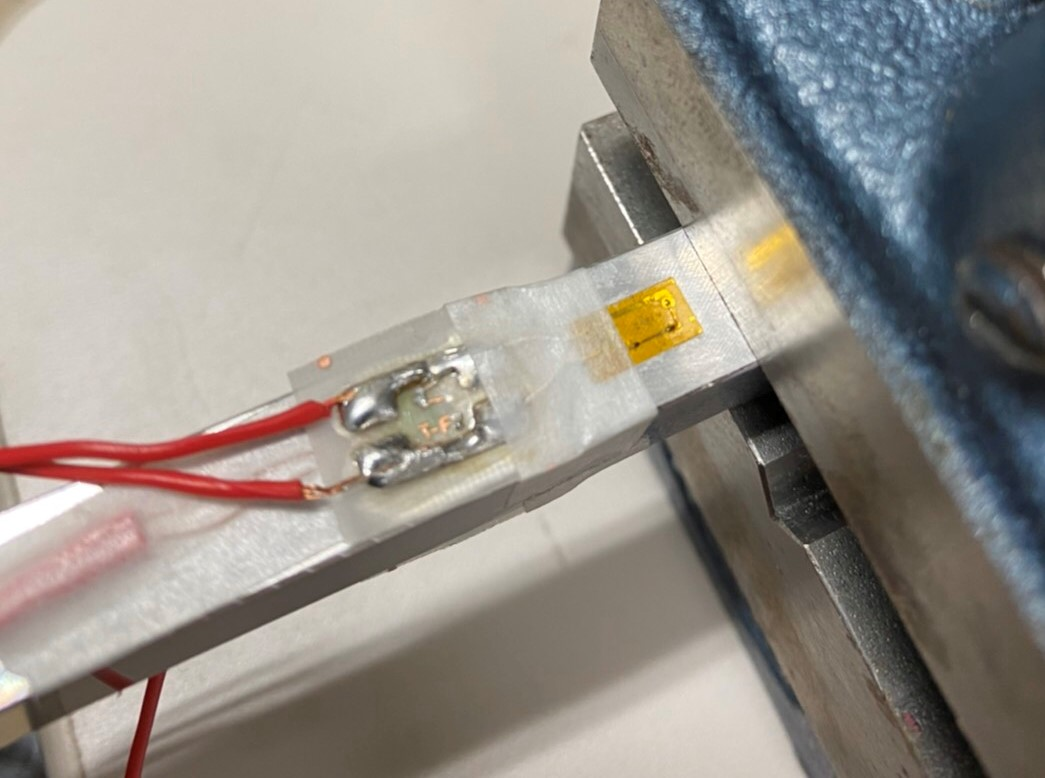
\includegraphics[scale=0.15]{pic/realSensor.jpg}
        \hspace{1.cm} 
        \footnotesize{製作したHDR1軸力覚センサ\\Made HDR unaxial force sensor}
      \end{center}
    \end{minipage}
        \begin{minipage}{0.51\hsize}
      \begin{center}
        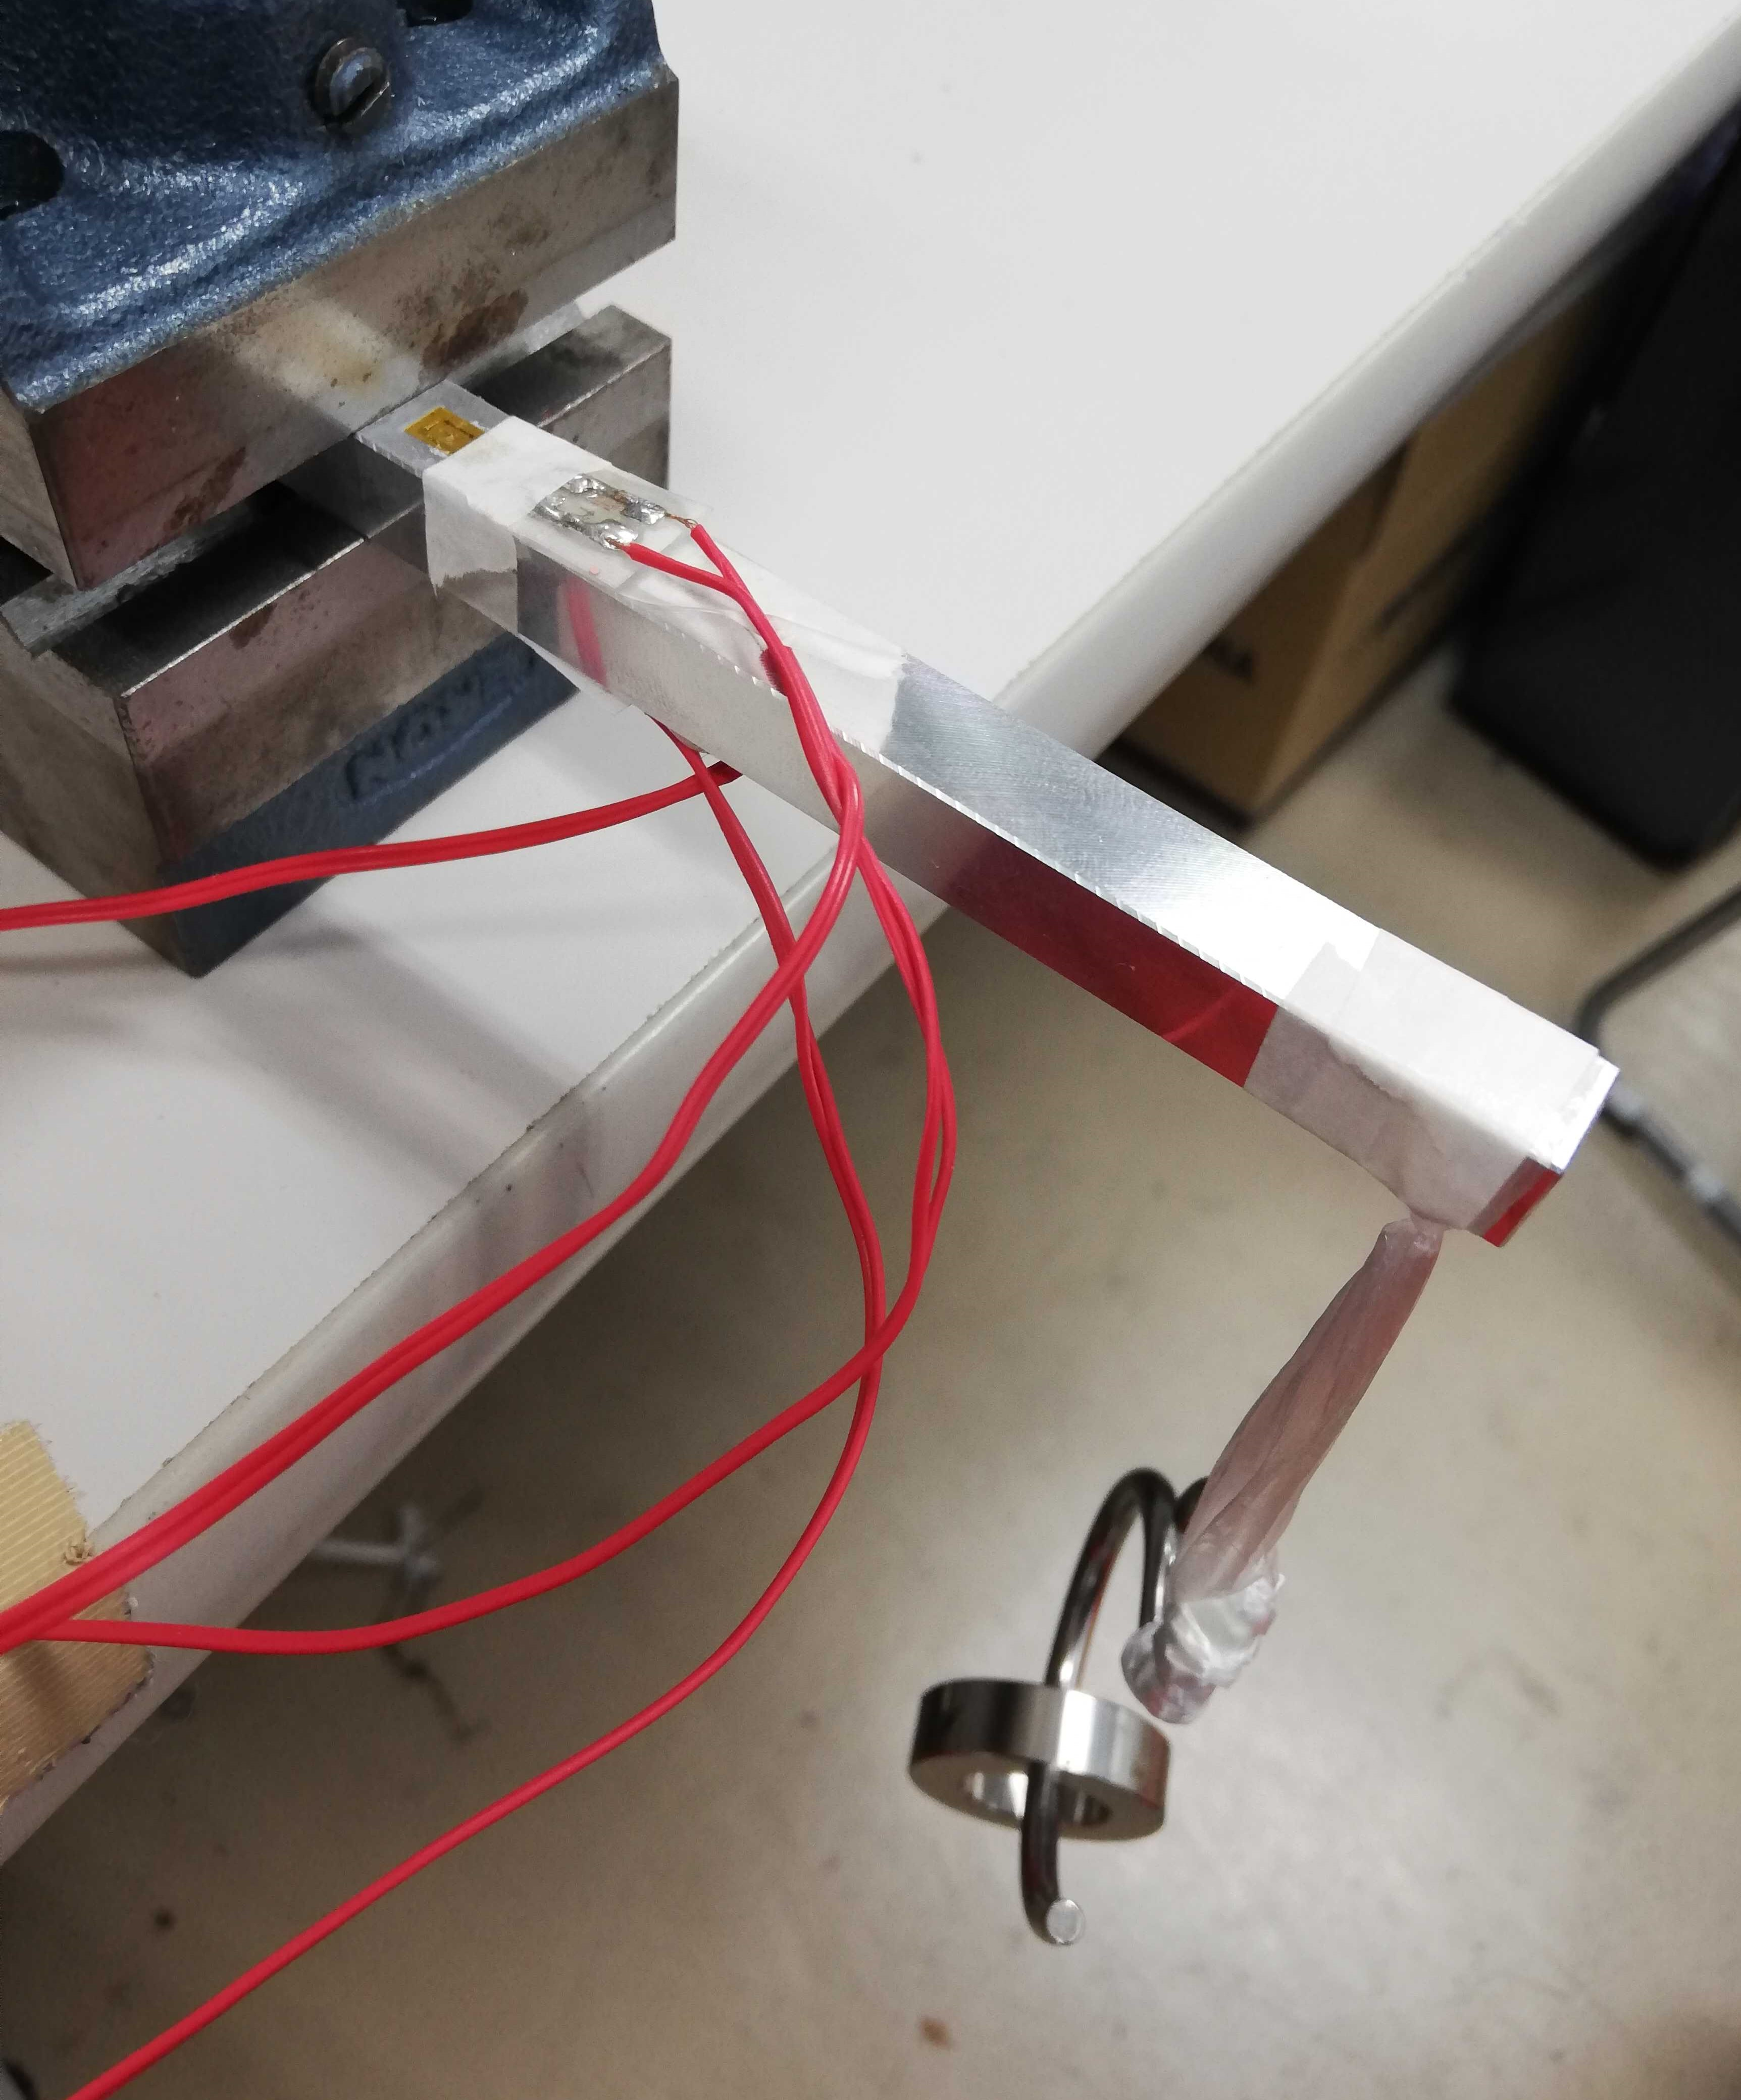
\includegraphics[scale=0.03]{pic/jikkenzu.jpg}
        \hspace{1.6cm} 
        \footnotesize{実験の様子\\State of experiment}
      \end{center}
    \end{minipage}
  \end{tabular}
  \caption[]{実際のHDR1軸力覚センサ\\Fig. 5 Actual HDR unaxial force sensor}\label{fig:jissai}
\end{figure}
さらに, 試験より得られた金属箔ひずみゲージの出力をFig.~\ref{fig:kinkeka}, 
半導体ひずみゲージの出力をFig.~\ref{fig:hankekka}に示す. 

Fig.~\ref{fig:kinkeka}, Fig.~\ref{fig:hankekka}を見比べると, 
同じ荷重を印加している時にそれぞれ出力が異なっていることが分かる. 
また, 半導体ひずみゲージの出力のほうが大きく得られていることから, 
低荷重に対し高感度に出力を得られることが確認できた. 

ここで, 1N印加時のシミュレーションによる起歪体自体のひずみ値と 
試験で得られた金属箔, 半導体ひずみゲージの出力を比較する. 
まず, シミューレーションにより1N印加時では
金属箔ひずみゲージ貼り付け位置:$6.658\mu$m/m, 
半導体ひずみゲージ貼り付け位置:$7.047\mu$m/m という結果が得られた. 
さらにFig.~\ref{fig:kinkeka}, Fig.~\ref{fig:hankekka}を見ると, 
金属箔ひずみゲージは無負荷時:$-3.21\mu$, 1N印加時:$8.62\mu$で
半導体ひずみゲージは無負荷時:$1.43\mu$, 1N印加時:$1358\mu$という結果が得られた.
ここで取り上げた数値は印加荷重に変動の無い一定時間の出力を平均したものである. 

金属箔ひずみゲージは無負荷時から1N印加時の間で約11.8$\mu$の変位がみられ,  
シミュレーションで得た起歪体のひずみ出力に対し, 約ゲージ率倍された出力が得られた.
また, 1N印加時の出力をもとに無負荷時のノイズによる出力値を荷重変換すると, 
約0.37Nであった. よって金属箔ひずみゲージでは約0.37N以上の
荷重であればノイズに埋もれることなく取得できる.

半導体ひずみゲージは無負荷時から1N印加時の間で約1357$\mu$の変位がみられる. 
シミュレーションで得た起歪体のひずみ出力に対し, 約ゲージ率倍された出力が得られた.
また, 1N印加時の出力をもとに無負荷時のノイズによる出力値を荷重変換すると, 
約0.001Nであった. よって半導体ひずみゲージでは約0.001N以上の
荷重であればノイズに埋もれることなく取得できる.

この結果より, 1つの起歪体上にゲージ率の異なるひずみゲージを張り付けることで, 
0.001Nから定格荷重である200Nまでの力覚情報の測定が
本センサで可能であることが示された. 

\begin{figure}[h]
  \begin{center}
    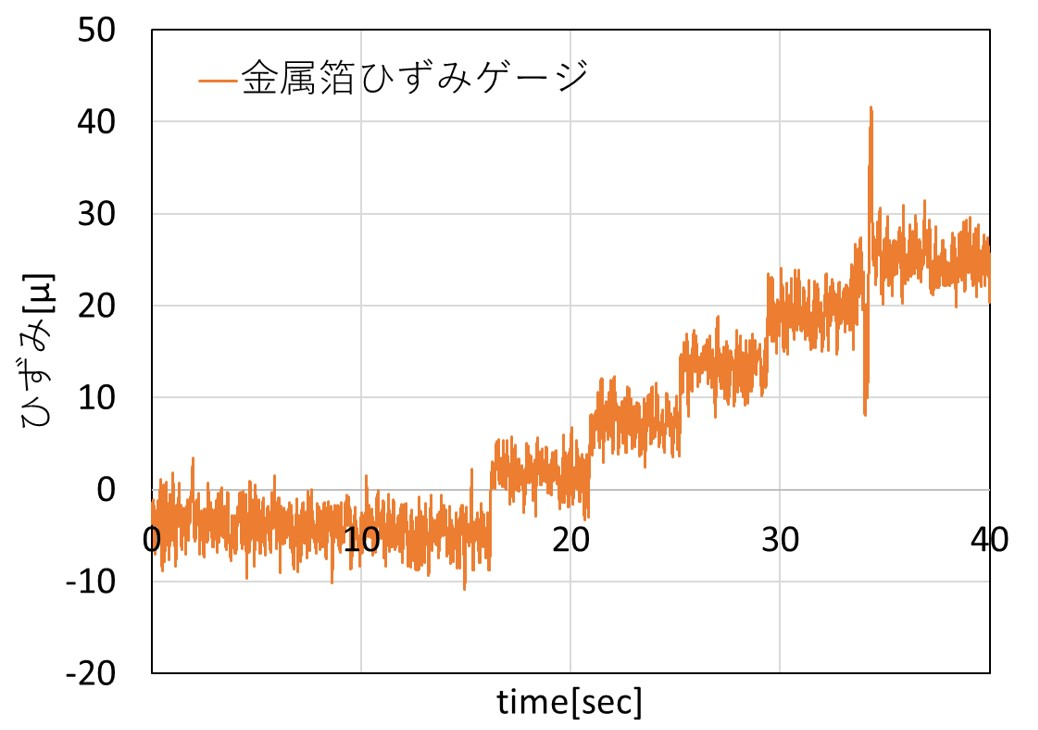
\includegraphics[width=8.0cm]{pic/kinkekka.jpg}
    \caption{金属箔ひずみゲージの出力\\Fig. 6 Output of metal foil strain gauge}\label{fig:kinkeka}
  \end{center}
\end{figure}

\begin{figure}[h]
  \begin{center}
    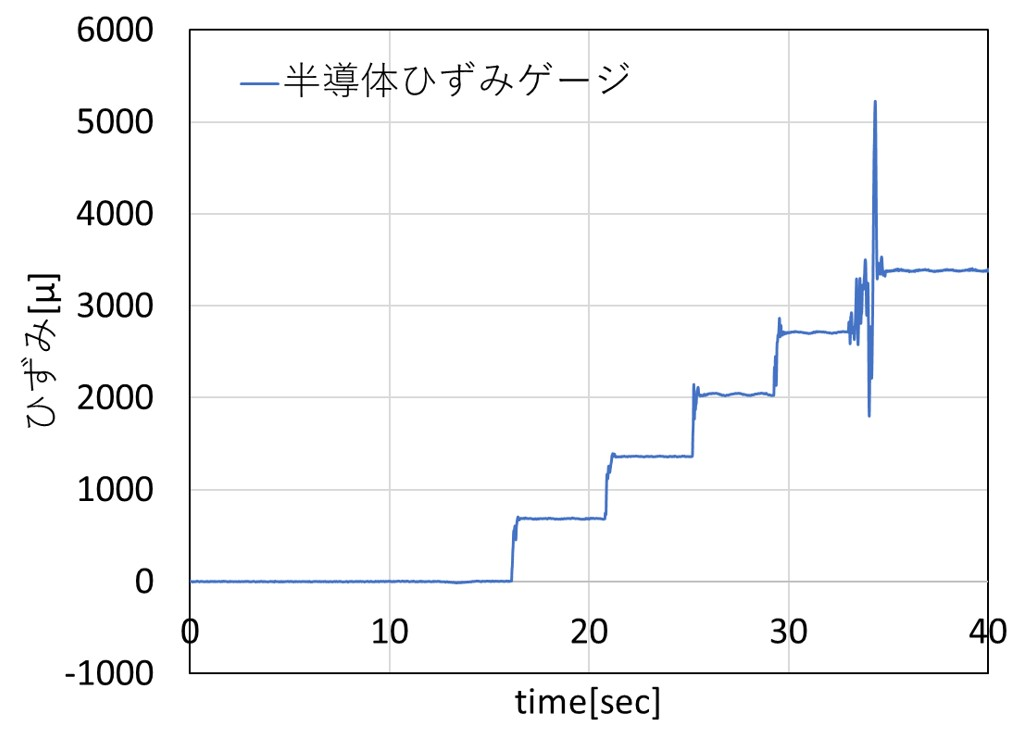
\includegraphics[width=8.0cm]{pic/hankekka.jpg}
    \caption{半導体ひずみゲージの出力\\Fig. 7 Output of semiconductor strain gauge}\label{fig:hankekka}
  \end{center}
\end{figure}